\documentclass[aspectratio=169]{beamer}

% Theme
\usetheme{Madrid}
\usecolortheme{default}

% Packages
\usepackage{tikz}
\usepackage{pgfplots}
\pgfplotsset{compat=1.18}
\usetikzlibrary{shapes.geometric, arrows.meta, positioning, calc}
\usepackage{booktabs}
\usepackage{graphicx}
\usepackage{amsmath}
\usepackage{xcolor}

% Custom colors
\definecolor{nkublue}{RGB}{0, 51, 102}
\definecolor{nkugold}{RGB}{204, 153, 0}

\setbeamercolor{structure}{fg=nkublue}
\setbeamercolor{title}{fg=white,bg=nkublue}
\setbeamercolor{frametitle}{fg=white,bg=nkublue}

% Remove navigation symbols
\setbeamertemplate{navigation symbols}{}

% Add frame numbers
\setbeamertemplate{footline}[frame number]

% Title information
\title[Multi-Agent RCA]{Multi-Agent Knowledge-Graph-Guided\\Root Cause Analysis}
\subtitle{Using Large Language Models for Reliable Log-Based Diagnosis}
\author{Zamo Rzgar Ahmed}
\institute[Nankai University]{
    College of Software\\
    Nankai University\\[1em]
    \textbf{Supervisor:} Prof. Sun Yongqian
}

\begin{document}

%==============================================================================
% SLIDE 1: Title
%==============================================================================
\begin{frame}
\titlepage
\end{frame}

%==============================================================================
% SLIDE 2: Outline
%==============================================================================
\begin{frame}{Outline}
\tableofcontents
\end{frame}

%==============================================================================
% SECTION 1: Introduction
%==============================================================================
\section{Introduction}

%==============================================================================
% SLIDE 3: Motivation
%==============================================================================
\begin{frame}{Motivation: The RCA Challenge}
\begin{columns}
\begin{column}{0.5\textwidth}
\textbf{Root Cause Analysis (RCA)} is critical for:
\begin{itemize}
    \item Diagnosing system failures
    \item Reducing downtime costs
    \item Preventing recurring incidents
\end{itemize}

\vspace{1em}
\textbf{Challenge:} Modern systems generate massive, heterogeneous logs that are difficult to analyze manually.
\end{column}
\begin{column}{0.5\textwidth}
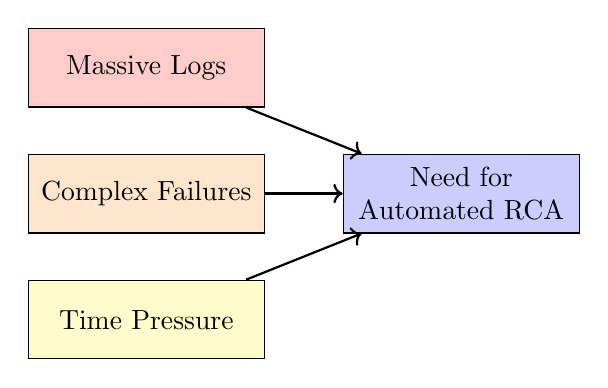
\begin{tikzpicture}[scale=0.8]
    \node[draw, rectangle, fill=red!20, minimum width=3cm, minimum height=1cm] (logs) at (0,2) {Massive Logs};
    \node[draw, rectangle, fill=orange!20, minimum width=3cm, minimum height=1cm] (complex) at (0,0) {Complex Failures};
    \node[draw, rectangle, fill=yellow!20, minimum width=3cm, minimum height=1cm] (time) at (0,-2) {Time Pressure};
    \node[draw, rectangle, fill=blue!20, minimum width=3cm, minimum height=1cm, align=center] (need) at (5,0) {Need for\\Automated RCA};
    \draw[->, thick] (logs) -- (need);
    \draw[->, thick] (complex) -- (need);
    \draw[->, thick] (time) -- (need);
\end{tikzpicture}
\end{column}
\end{columns}
\end{frame}

%==============================================================================
% SLIDE 4: Problem with Single-LLM
%==============================================================================
\begin{frame}{Problem: Single-LLM Limitations}
\begin{columns}
\begin{column}{0.55\textwidth}
\textbf{Single-LLM approaches suffer from:}
\vspace{0.5em}
\begin{enumerate}
    \item \textbf{Hallucinations}
    \begin{itemize}
        \item Making claims not grounded in evidence
        \item Inventing non-existent error patterns
    \end{itemize}
    \vspace{0.3em}
    \item \textbf{Tunnel Vision}
    \begin{itemize}
        \item Missing alternative explanations
        \item Fixating on first hypothesis
    \end{itemize}
    \vspace{0.3em}
    \item \textbf{No Verification}
    \begin{itemize}
        \item No cross-checking mechanism
        \item No evidence-based selection
    \end{itemize}
\end{enumerate}
\end{column}
\begin{column}{0.45\textwidth}
\centering
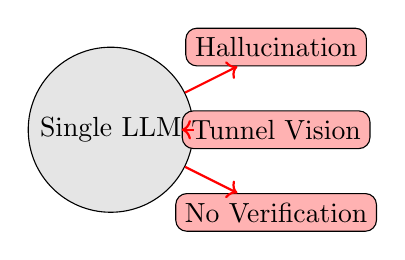
\begin{tikzpicture}[scale=0.7]
    \node[draw, circle, fill=gray!20, minimum size=2cm] (llm) at (0,0) {Single LLM};
    \node[draw, rectangle, fill=red!30, minimum width=2cm, rounded corners] (h1) at (3,1.5) {Hallucination};
    \node[draw, rectangle, fill=red!30, minimum width=2cm, rounded corners] (h2) at (3,0) {Tunnel Vision};
    \node[draw, rectangle, fill=red!30, minimum width=2cm, rounded corners] (h3) at (3,-1.5) {No Verification};
    \draw[->, thick, red] (llm) -- (h1);
    \draw[->, thick, red] (llm) -- (h2);
    \draw[->, thick, red] (llm) -- (h3);
\end{tikzpicture}
\end{column}
\end{columns}
\end{frame}

%==============================================================================
% SLIDE 5: Research Questions
%==============================================================================
\begin{frame}{Research Questions}
\begin{block}{RQ1: Accuracy}
Does multi-agent KG-guided RCA achieve higher accuracy than single-agent and RAG baselines?
\end{block}

\begin{block}{RQ2: Cross-Domain Generalization}
Can the system generalize across different log datasets without dataset-specific training?
\end{block}

\begin{block}{RQ3: Debate Effectiveness}
Does the multi-agent debate protocol improve hypothesis quality over single-pass generation?
\end{block}

\begin{block}{RQ4: Knowledge Graph Value}
Does KG-based historical context improve diagnostic accuracy?
\end{block}
\end{frame}

%==============================================================================
% SECTION 2: System Design
%==============================================================================
\section{System Design}

%==============================================================================
% SLIDE 6: Architecture Overview
%==============================================================================
\begin{frame}{System Architecture}
\centering
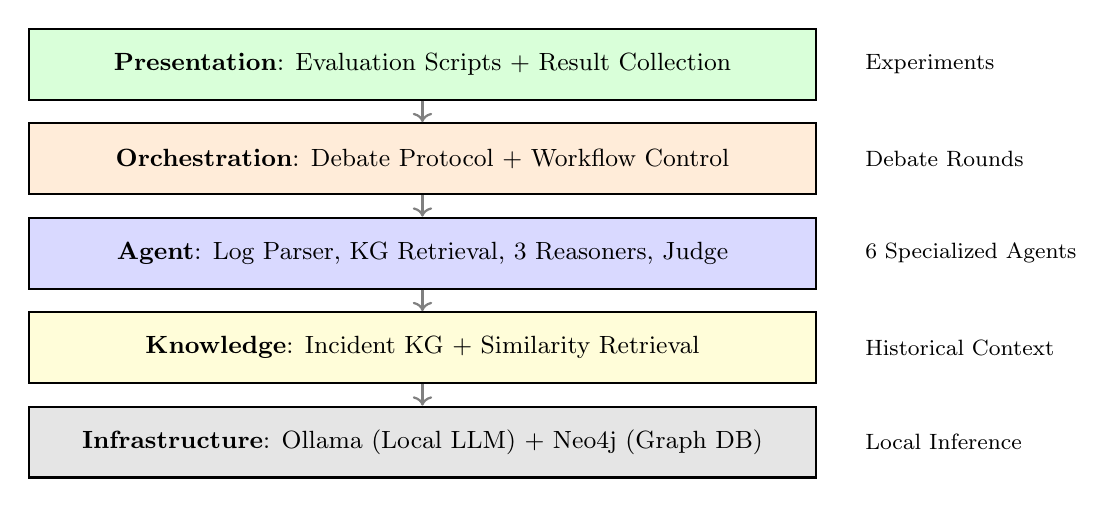
\begin{tikzpicture}[node distance=0.5cm, font=\small,
    layer/.style={rectangle, draw=black, thick, minimum width=10cm, minimum height=0.9cm, align=center}
]
% Layers (bottom to top)
\node[layer, fill=gray!20] (infra) at (0,0) {\textbf{Infrastructure}: Ollama (Local LLM) + Neo4j (Graph DB)};
\node[layer, fill=yellow!15] (knowledge) at (0,1.2) {\textbf{Knowledge}: Incident KG + Similarity Retrieval};
\node[layer, fill=blue!15] (agent) at (0,2.4) {\textbf{Agent}: Log Parser, KG Retrieval, 3 Reasoners, Judge};
\node[layer, fill=orange!15] (orch) at (0,3.6) {\textbf{Orchestration}: Debate Protocol + Workflow Control};
\node[layer, fill=green!15] (pres) at (0,4.8) {\textbf{Presentation}: Evaluation Scripts + Result Collection};

% Arrows
\draw[->, thick, gray] (pres.south) -- (orch.north);
\draw[->, thick, gray] (orch.south) -- (agent.north);
\draw[->, thick, gray] (agent.south) -- (knowledge.north);
\draw[->, thick, gray] (knowledge.south) -- (infra.north);

% Labels
\node[anchor=west, font=\footnotesize] at (5.5,4.8) {Experiments};
\node[anchor=west, font=\footnotesize] at (5.5,3.6) {Debate Rounds};
\node[anchor=west, font=\footnotesize] at (5.5,2.4) {6 Specialized Agents};
\node[anchor=west, font=\footnotesize] at (5.5,1.2) {Historical Context};
\node[anchor=west, font=\footnotesize] at (5.5,0) {Local Inference};
\end{tikzpicture}
\end{frame}

%==============================================================================
% SLIDE 7: Pipeline Flow
%==============================================================================
\begin{frame}{Multi-Agent Pipeline}
\centering
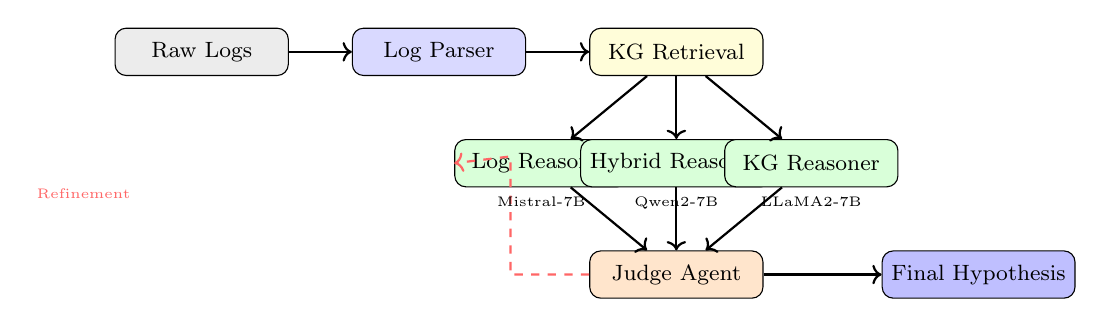
\begin{tikzpicture}[node distance=0.6cm, font=\footnotesize,
    box/.style={draw, rounded corners, align=center, minimum width=2.2cm, minimum height=0.6cm}
]
  \node[box, fill=gray!15] (logs) {Raw Logs};
  \node[box, fill=blue!15, right=0.8cm of logs] (parser) {Log Parser};
  \node[box, fill=yellow!15, right=0.8cm of parser] (kg) {KG Retrieval};
  
  \node[box, fill=green!15, below left=0.8cm and -0.5cm of kg] (logr) {Log Reasoner};
  \node[box, fill=green!15, below=0.8cm of kg] (hyb) {Hybrid Reasoner};
  \node[box, fill=green!15, below right=0.8cm and -0.5cm of kg] (kgr) {KG Reasoner};
  
  \node[box, fill=orange!20, below=0.8cm of hyb] (judge) {Judge Agent};
  \node[box, fill=blue!25, right=1.5cm of judge] (out) {Final Hypothesis};

  \draw[->, thick] (logs) -- (parser);
  \draw[->, thick] (parser) -- (kg);
  \draw[->, thick] (kg) -- (logr);
  \draw[->, thick] (kg) -- (hyb);
  \draw[->, thick] (kg) -- (kgr);
  \draw[->, thick] (logr) -- (judge);
  \draw[->, thick] (hyb) -- (judge);
  \draw[->, thick] (kgr) -- (judge);
  \draw[->, thick] (judge) -- (out);
  
  % Feedback loop
  \draw[->, dashed, thick, red!60] (judge.west) -- ++(-1,0) -- ++(0,1.5) -- (logr.west);
  \node[font=\tiny, red!60] at (-1.5,-1.8) {Refinement};
  
  % Annotations
  \node[font=\tiny, anchor=north] at (logr.south) {Mistral-7B};
  \node[font=\tiny, anchor=north] at (hyb.south) {Qwen2-7B};
  \node[font=\tiny, anchor=north] at (kgr.south) {LLaMA2-7B};
\end{tikzpicture}

\vspace{0.5em}
\textbf{Key Innovation:} Three diverse reasoners generate competing hypotheses; Judge selects best one based on evidence.
\end{frame}

%==============================================================================
% SLIDE 8: Debate Protocol
%==============================================================================
\begin{frame}{Multi-Agent Debate Protocol}
\begin{columns}
\begin{column}{0.5\textwidth}
\textbf{Debate Flow (up to 3 rounds):}
\begin{enumerate}
    \item \textbf{Generation}: Each reasoner produces 3-5 hypotheses
    \item \textbf{Judging}: Judge scores all hypotheses (0-100)
    \item \textbf{Feedback}: Detailed critique with strengths/weaknesses
    \item \textbf{Refinement}: Reasoners improve based on feedback
    \item \textbf{Convergence}: Stop when scores plateau
\end{enumerate}

\vspace{0.5em}
\textbf{Scoring Criteria:}
\begin{itemize}
    \item Evidence support (40\%)
    \item Logical coherence (30\%)
    \item Specificity (20\%)
    \item Actionability (10\%)
\end{itemize}
\end{column}
\begin{column}{0.5\textwidth}
\centering
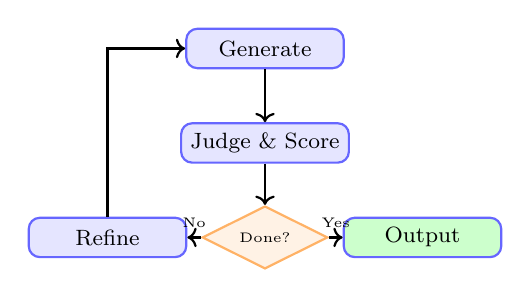
\begin{tikzpicture}[node distance=0.6cm, font=\footnotesize,
    process/.style={rectangle, draw=blue!60, fill=blue!10, thick, minimum width=2cm, minimum height=0.5cm, align=center, rounded corners},
    decision/.style={diamond, draw=orange!60, fill=orange!10, thick, minimum width=0.8cm, align=center, aspect=2, font=\tiny}
]
\node[process] (gen) at (0,0) {Generate};
\node[process] (judge) at (0,-1.2) {Judge \& Score};
\node[decision] (conv) at (0,-2.4) {Done?};
\node[process] (refine) at (-2,-2.4) {Refine};
\node[process, fill=green!20] (output) at (2,-2.4) {Output};

\draw[->, thick] (gen) -- (judge);
\draw[->, thick] (judge) -- (conv);
\draw[->, thick] (conv) -- node[above, font=\tiny] {Yes} (output);
\draw[->, thick] (conv) -- node[above, font=\tiny] {No} (refine);
\draw[->, thick] (refine) |- (gen);
\end{tikzpicture}
\end{column}
\end{columns}
\end{frame}

%==============================================================================
% SLIDE 9: Knowledge Graph
%==============================================================================
\begin{frame}{Knowledge Graph for Historical Context}
\begin{columns}
\begin{column}{0.55\textwidth}
\textbf{KG Structure:}
\begin{itemize}
    \item \textbf{Nodes}: Incidents, Components, Error Types, Root Causes
    \item \textbf{Edges}: CAUSED\_BY, INVOLVES, SIMILAR\_TO
    \item \textbf{Storage}: Neo4j graph database
\end{itemize}

\vspace{0.5em}
\textbf{Retrieval Process:}
\begin{enumerate}
    \item Extract entities from current incident
    \item Query KG for similar historical incidents
    \item Retrieve past diagnoses and resolutions
    \item Provide context to reasoners
\end{enumerate}

\vspace{0.5em}
\textbf{Benefit}: Grounds reasoning in historical evidence, reduces hallucinations.
\end{column}
\begin{column}{0.45\textwidth}
\centering
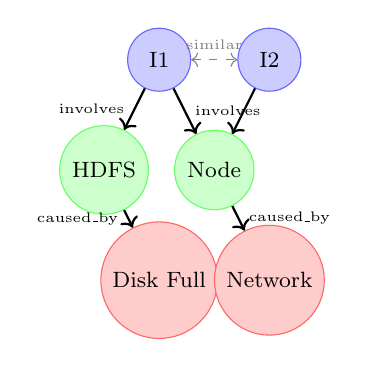
\begin{tikzpicture}[scale=0.7, font=\footnotesize,
    incident/.style={circle, draw=blue!60, fill=blue!20, minimum size=0.8cm},
    component/.style={circle, draw=green!60, fill=green!20, minimum size=0.8cm},
    cause/.style={circle, draw=red!60, fill=red!20, minimum size=0.8cm}
]
\node[incident] (i1) at (0,2) {I1};
\node[incident] (i2) at (2,2) {I2};
\node[component] (c1) at (-1,0) {HDFS};
\node[component] (c2) at (1,0) {Node};
\node[cause] (r1) at (0,-2) {Disk Full};
\node[cause] (r2) at (2,-2) {Network};

\draw[->, thick] (i1) -- node[left, font=\tiny] {involves} (c1);
\draw[->, thick] (i1) -- node[right, font=\tiny] {involves} (c2);
\draw[->, thick] (i2) -- (c2);
\draw[->, thick] (c1) -- node[left, font=\tiny] {caused\_by} (r1);
\draw[->, thick] (c2) -- node[right, font=\tiny] {caused\_by} (r2);
\draw[<->, dashed, gray] (i1) -- node[above, font=\tiny] {similar} (i2);
\end{tikzpicture}

\vspace{0.3em}
\textbf{Legend:} \textcolor{blue!60}{Incident} \textcolor{green!60}{Component} \textcolor{red!60}{Root Cause}
\end{column}
\end{columns}
\end{frame}

%==============================================================================
% SECTION 3: Evaluation
%==============================================================================
\section{Evaluation}

%==============================================================================
% SLIDE 10: Datasets
%==============================================================================
\begin{frame}{Evaluation Datasets}
\begin{table}
\centering
\begin{tabular}{lccc}
\toprule
\textbf{Dataset} & \textbf{Cases} & \textbf{Classes} & \textbf{Domain} \\
\midrule
Hadoop1 (LogHub) & 55 & 4 fault types & Distributed computing \\
CMCC (LogKG) & 93 & 7 failure types & OpenStack cloud \\
HDFS\_v1 (LogHub) & 200 & 2 (normal/anomaly) & Storage system \\
\bottomrule
\end{tabular}
\end{table}

\vspace{1em}
\textbf{Evaluation Protocol:}
\begin{itemize}
    \item Zero-shot evaluation (no dataset-specific training)
    \item Macro-F1 as primary metric (handles class imbalance)
    \item Compare: Multi-Agent vs. RAG vs. Single-Agent
\end{itemize}
\end{frame}

%==============================================================================
% SLIDE 11: Results Table
%==============================================================================
\begin{frame}{Experimental Results}
\begin{table}
\centering
\large
\begin{tabular}{l|ccc}
\toprule
\textbf{Dataset} & \textbf{Multi-Agent} & \textbf{RAG} & \textbf{Single-Agent} \\
\midrule
Hadoop1 (Coarse) & \textbf{39.1\%} & 37.9\% & 25.8\% \\
CMCC & \textbf{52.4\%} & 7.8\% & 3.9\% \\
HDFS\_v1 & \textbf{69.4\%} & 63.0\% & 56.8\% \\
\bottomrule
\end{tabular}
\caption{Macro-F1 scores across all datasets}
\end{table}

\vspace{0.5em}
\begin{block}{Key Findings}
\begin{itemize}
    \item Multi-agent \textbf{consistently outperforms} baselines on all datasets
    \item Largest improvement on CMCC: \textbf{+48.5 pp} over single-agent
    \item KG retrieval (RAG) helps, but debate provides additional gains
\end{itemize}
\end{block}
\end{frame}

%==============================================================================
% SLIDE 12: Results Chart
%==============================================================================
\begin{frame}{Results Comparison}
\centering
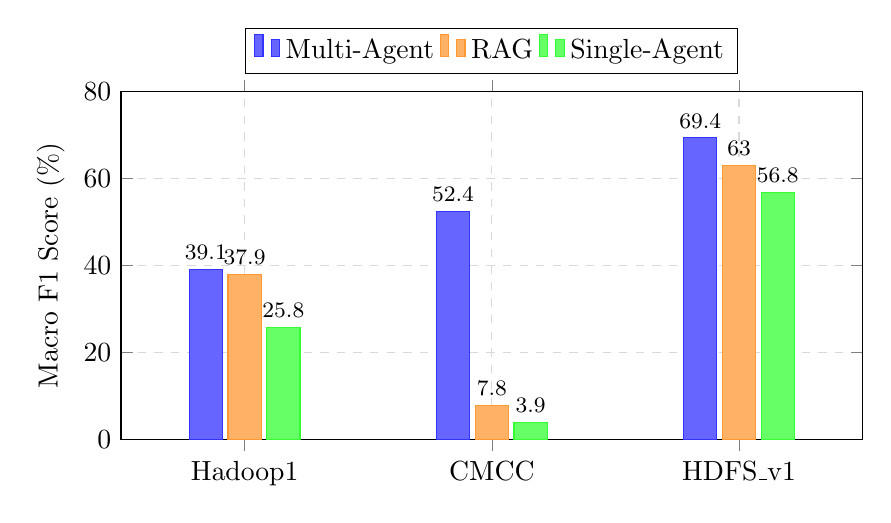
\begin{tikzpicture}
\begin{axis}[
    ybar,
    bar width=12pt,
    width=11cm,
    height=6cm,
    ylabel={Macro F1 Score (\%)},
    ymin=0,
    ymax=80,
    xtick=data,
    symbolic x coords={Hadoop1, CMCC, HDFS\_v1},
    legend style={at={(0.5,1.05)}, anchor=south, legend columns=3},
    nodes near coords,
    nodes near coords align={vertical},
    every node near coord/.append style={font=\footnotesize},
    enlarge x limits=0.25,
    grid=major,
    grid style={dashed, gray!30},
]
\addplot[fill=blue!60, draw=blue!80] coordinates {
    (Hadoop1, 39.1)
    (CMCC, 52.4)
    (HDFS\_v1, 69.4)
};
\addplot[fill=orange!60, draw=orange!80] coordinates {
    (Hadoop1, 37.9)
    (CMCC, 7.8)
    (HDFS\_v1, 63.0)
};
\addplot[fill=green!60, draw=green!80] coordinates {
    (Hadoop1, 25.8)
    (CMCC, 3.9)
    (HDFS\_v1, 56.8)
};
\legend{Multi-Agent, RAG, Single-Agent}
\end{axis}
\end{tikzpicture}
\end{frame}

%==============================================================================
% SLIDE 13: Analysis
%==============================================================================
\begin{frame}{Why Multi-Agent Works Better}
\begin{columns}
\begin{column}{0.5\textwidth}
\textbf{1. Diversity of Perspectives}
\begin{itemize}
    \item Log Reasoner: Pattern-focused
    \item KG Reasoner: History-focused
    \item Hybrid: Balanced approach
\end{itemize}

\vspace{0.5em}
\textbf{2. Verification Mechanism}
\begin{itemize}
    \item Judge evaluates evidence quality
    \item Rejects unsupported claims
    \item Reduces hallucinations
\end{itemize}
\end{column}
\begin{column}{0.5\textwidth}
\textbf{3. Iterative Refinement}
\begin{itemize}
    \item Feedback improves hypotheses
    \item Cross-pollination of ideas
    \item Convergence to better answers
\end{itemize}

\vspace{0.5em}
\textbf{4. KG Grounding}
\begin{itemize}
    \item Historical context reduces guessing
    \item Similar incidents guide reasoning
    \item Evidence-based diagnosis
\end{itemize}
\end{column}
\end{columns}

\vspace{1em}
\begin{alertblock}{CMCC Result Explained}
Single-agent and RAG collapse to ``unknown'' predictions on CMCC's complex OpenStack failures. Multi-agent's debate mechanism enables recovery through iterative refinement.
\end{alertblock}
\end{frame}

%==============================================================================
% SECTION 4: Contributions
%==============================================================================
\section{Contributions}

%==============================================================================
% SLIDE 14: Contributions
%==============================================================================
\begin{frame}{Contributions}
\begin{enumerate}
    \item \textbf{Novel Multi-Agent Architecture}
    \begin{itemize}
        \item First system combining multi-agent debate with KG grounding for log-based RCA
        \item Three specialized reasoners with complementary perspectives
    \end{itemize}
    
    \vspace{0.5em}
    \item \textbf{Structured Debate Protocol}
    \begin{itemize}
        \item Evidence-based hypothesis scoring
        \item Iterative refinement with feedback
        \item Convergence-aware stopping criteria
    \end{itemize}
    
    \vspace{0.5em}
    \item \textbf{Comprehensive Evaluation}
    \begin{itemize}
        \item Three diverse datasets (Hadoop, OpenStack, HDFS)
        \item Comparison with single-agent and RAG baselines
        \item Analysis of failure modes and improvements
    \end{itemize}
    
    \vspace{0.5em}
    \item \textbf{Fully Local Implementation}
    \begin{itemize}
        \item Runs on local hardware via Ollama
        \item No external API dependencies
        \item Reproducible and privacy-preserving
    \end{itemize}
\end{enumerate}
\end{frame}

%==============================================================================
% SLIDE 15: Conclusion & Future Work
%==============================================================================
\begin{frame}{Conclusion \& Future Work}
\begin{block}{Conclusion}
\begin{itemize}
    \item Multi-agent debate with KG grounding \textbf{improves RCA accuracy}
    \item Consistent improvements across \textbf{three diverse datasets}
    \item Largest gains on complex, cross-domain failures (CMCC: +48.5 pp)
    \item Verification mechanism \textbf{reduces hallucinations}
\end{itemize}
\end{block}

\vspace{0.5em}
\begin{block}{Future Work}
\begin{itemize}
    \item \textbf{Larger models}: Evaluate with 13B+ parameter models
    \item \textbf{Fine-tuning}: Domain-specific adaptation via LoRA/QLoRA
    \item \textbf{Real-time deployment}: Integration with monitoring systems
    \item \textbf{Human-in-the-loop}: Interactive refinement with operators
\end{itemize}
\end{block}
\end{frame}

%==============================================================================
% SLIDE 16: Thank You
%==============================================================================
\begin{frame}
\centering
\vspace{2em}
{\Huge \textbf{Thank You!}}

\vspace{2em}
{\Large Questions?}

\vspace{3em}
\textbf{Zamo Rzgar Ahmed}\\
College of Software, Nankai University\\
Supervisor: Prof. Sun Yongqian
\end{frame}

\end{document}
